\documentclass[11pt]{article}
\usepackage{amsmath, amssymb, physics, mathtools, bm}
\usepackage{tikz, pgfplots}
\pgfplotsset{compat=1.18}
\usepackage[margin=2.3cm]{geometry}
\usepackage{siunitx, booktabs, hyperref}
\usepackage{braket}

\newcommand{\D}{\mathrm{D}}
\newcommand{\de}{\mathrm{d}}
\newcommand{\pd}[2]{\frac{\partial #1}{\partial #2}}
\newcommand{\pdd}[2]{\frac{\partial^{2} #1}{\partial #2^{2}}}
\newcommand{\Lap}{\nabla^{2}}

\title{B1 Flows, Fluctuations and Complexity --- Model Solutions, 2018}
\author{}
\date{}

\begin{document}
\maketitle

%==========================================================
\section*{Question 1 --- Bernoulli and wind over ripples}

\subsection*{(a) Bernoulli's theorem}

\textbf{Problem.} Derive the conserved quantity along streamlines of a steady, inviscid, incompressible, irrotational flow under gravity from Navier--Stokes; identify each term; comment on the compressible case.

Drop $\nu\Lap\vb u$ (inviscid) and $\partial_t\vb u$ (steady) from N--S:
\[
(\vb u\cdot\nabla)\vb u + \tfrac{1}{\rho}\nabla p + g\hat{\vb k} = 0.
\]
Apply identity $(\vb u\cdot\nabla)\vb u = \nabla(|\vb u|^2/2) - \vb u\times(\nabla\times\vb u)$:
\[
\nabla\!\left(\tfrac{|\vb u|^2}{2}\right) - \vb u\times\bm\omega + \tfrac{1}{\rho}\nabla p + g\hat{\vb k} = 0,\qquad \bm\omega = \nabla\times\vb u.
\]
Irrotational flow: $\bm\omega = 0$:
\[
\nabla\!\left(\tfrac{|\vb u|^2}{2} + \tfrac{p}{\rho} + g z\right) = 0.
\]
Integrate:
\[
\boxed{\;\tfrac{1}{2}|\vb u|^2 + \tfrac{p}{\rho} + g z = \text{const everywhere}\;}
\]

Origin of terms: $\tfrac{1}{2}|\vb u|^2$ is kinetic energy per unit mass (advective term); $p/\rho$ is the work done by pressure forces per unit mass (pressure term); $gz$ is gravitational potential energy per unit mass.

Compressible interpretation: with $\rho = \rho(p)$, $\nabla p/\rho$ is no longer $\nabla(p/\rho)$. The pressure term must be replaced by the enthalpy $\int \de p/\rho(p)$, which becomes $c_p T$ for an ideal gas. Bernoulli then expresses conservation of total enthalpy along a streamline.

\subsection*{(b) Air flow over rippled water}

\textbf{Problem.} Justify irrotationality; show $u = U_0[1 + a\sin(2\pi x/\lambda)e^{-bz}]$ is consistent with incompressibility and the BCs above $h = \eta\sin(2\pi x/\lambda)$; find $a, b$; sketch streamlines.

Irrotationality: at $x<0$ the flow is uniform, hence $\bm\omega=0$. With $\nu_\text{air}\to 0$, the vorticity equation $\D\bm\omega/\D t = (\bm\omega\cdot\nabla)\vb u$ has no source, so $\bm\omega = 0$ is preserved along streamlines downstream of $x=0$.

Let $k = 2\pi/\lambda$. Incompressibility:
\[
\partial_x u + \partial_z w = 0.
\]
Compute $\partial_x u$:
\[
\partial_x u = U_0 a k \cos(kx)\,e^{-bz}.
\]
Integrate $-\partial_x u$ in $z$ for $w$:
\[
w = -\int \partial_x u\,\de z = \tfrac{U_0 a k}{b}\cos(kx)\,e^{-bz} + C(x).
\]
Far-field BC $w\to 0$ as $z\to\infty$: $C(x) = 0$:
\[
w(x,z) = \tfrac{U_0 a k}{b}\cos(kx)\,e^{-bz}.
\]
Kinematic BC at $z=0$ (linearised, since $\eta\ll\lambda$ and phase speed $\ll U_0$, hence steady):
\[
w(x,0) = U_0\,\partial_x h = U_0\,\eta k\,\cos(kx).
\]
Match coefficients:
\[
\tfrac{U_0 a k}{b}\cos(kx) = U_0\,\eta k\,\cos(kx).
\]
Solve for $a$:
\[
a = \tfrac{\eta b}{1} \cdot \tfrac{1}{1} \;\Rightarrow\; a = \eta b. \tag{i}
\]
Irrotationality $\partial_z u - \partial_x w = 0$:
\[
-U_0 a b\sin(kx)e^{-bz} - \bigl(-\tfrac{U_0 a k^2}{b}\sin(kx)e^{-bz}\bigr) = 0.
\]
Cancel common factor:
\[
-a b + \tfrac{a k^2}{b} = 0.
\]
Solve for $b$:
\[
b^2 = k^2 \;\Rightarrow\; b = k = \tfrac{2\pi}{\lambda}.
\]
Substitute into (i):
\[
\boxed{\;a = \eta k = \tfrac{2\pi\eta}{\lambda},\qquad b = k = \tfrac{2\pi}{\lambda}\;}
\]

Boundary conditions used: (1) $w\to 0$ as $z\to\infty$ (undisturbed flow far above); (2) $w(x,0) = U_0\,\partial_x h$ (kinematic, linearised); (3) $u\to U_0$ as $z\to\infty$.

Streamline sketch:

\begin{center}
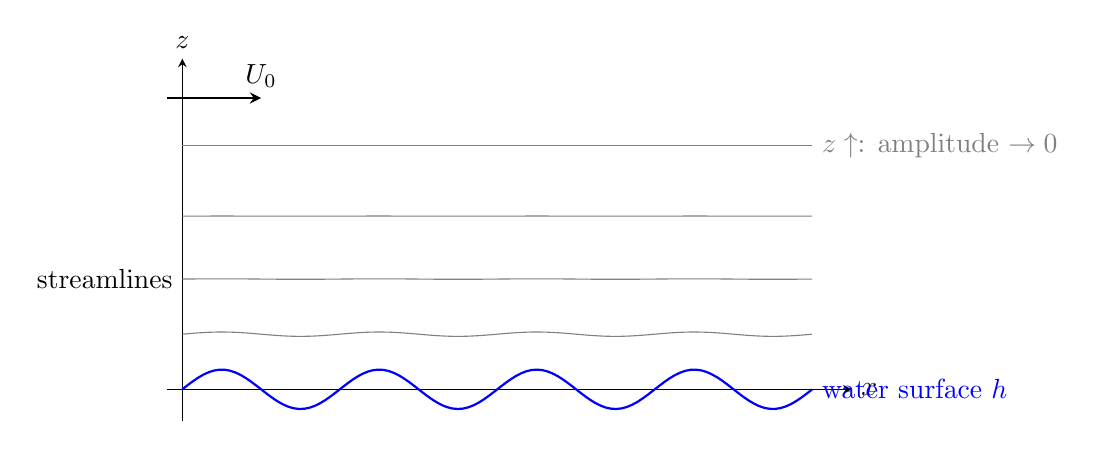
\begin{tikzpicture}[>=stealth, scale=1.0]
  \draw[->] (-0.2,0) -- (8.5,0) node[right] {$x$};
  \draw[->] (0,-0.4) -- (0,4.2) node[above] {$z$};
  % water surface
  \draw[thick, blue] plot[domain=0:8, samples=120] (\x, {0.25*sin(deg(2*pi*\x/2))});
  \node[blue, right] at (8, 0) {water surface $h$};
  % streamlines (decay with z, in phase with surface near z=0)
  \foreach \z in {0.7, 1.4, 2.2, 3.1} {
    \draw[gray] plot[domain=0:8, samples=120] (\x, {\z + 0.25*exp(-2*pi*\z/2)*sin(deg(2*pi*\x/2))});
  }
  \node[gray, right] at (8, 3.1) {$z\uparrow$: amplitude $\to 0$};
  \node[left] at (0, 1.4) {streamlines};
  \draw[->, thick] (-0.2, 3.7) -- (1.0, 3.7) node[above] {$U_0$};
\end{tikzpicture}
\end{center}

Streamlines mirror the surface near $z=0$ and flatten exponentially with decay length $1/k = \lambda/(2\pi)$.

\subsection*{(c) Pressure at surface; ripple growth}

\textbf{Problem.} Find $p$ at $z=0$; explain how a steady wind grows ripples even with inviscid air; does the mechanism depend on direction of propagation; two amplitude-limiting processes.

Bernoulli on surface streamline ($z\approx 0$, drop $gz$ since linearisation is in air, the $g$ term is the same constant on the surface):
\[
p + \tfrac{1}{2}\rho_a |\vb u|^2 = p_\infty + \tfrac{1}{2}\rho_a U_0^2.
\]
At $z=0$, $u = U_0[1 + a\sin(kx)]$, $w = (U_0 a k/b)\cos(kx) = U_0 a\cos(kx)$:
\[
|\vb u|^2 = U_0^2\bigl[(1 + a\sin kx)^2 + a^2\cos^2 kx\bigr].
\]
Linearise in $a = \eta k \ll 1$:
\[
|\vb u|^2 \approx U_0^2\bigl[1 + 2a\sin(kx)\bigr].
\]
Substitute:
\[
p(x,0) = p_\infty - \rho_a U_0^2\,a\sin(kx).
\]
Insert $a = \eta k$:
\[
\boxed{\;p(x,0) = p_\infty - \rho_a U_0^2\,\eta k\,\sin(kx)\;}
\]

Phase relation: surface elevation is $h = \eta\sin(kx)$; pressure perturbation is $\delta p = -\rho_a U_0^2 \eta k\sin(kx)$. Pressure is \emph{lowest at the crests} ($\sin kx = +1$) and \emph{highest at the troughs} ($\sin kx = -1$). This pressure pattern is in antiphase with the displacement, which alone would not transfer energy (energy transfer requires a pressure component in phase with the surface velocity).

For energy transfer, allow ripples to propagate with phase speed $c\ll U_0$: $h = \eta\sin(k(x - ct))$. The kinematic BC then becomes $w(x,0) = (U_0 - c)\,\partial_x h$, so the pressure perturbation acquires a small $\cos$-component proportional to $c/U_0$ that is in phase with $\partial_t h$. The wind does positive work on the surface, transferring energy from the air to the water and amplifying the ripple. This is the inviscid Miles--type instability mechanism.

Direction dependence: yes. Reversing the propagation direction ($c \to -c$) flips the sign of the work integral $\oint p\,\partial_t h\,\de x$, so wind amplifies only ripples propagating in the same sense as $U_0$; counter-propagating ripples are damped.

Amplitude-limiting processes (any two): (1) viscous dissipation in the water (and the thin air boundary layer); (2) nonlinear wave breaking / whitecapping once $\eta k \sim 1$; (3) energy transfer by nonlinear wave--wave interactions to other wavenumbers; (4) surface tension increasing the restoring force as $k$ grows.

%==========================================================
\section*{Question 2 --- Pipe flow}

\subsection*{(a) Definitions}

\textbf{Problem.} Define steady, axisymmetric, fully developed flow.

Steady: $\partial_t\vb u = 0$. Axisymmetric: $\partial_\Theta\vb u = 0$, with $u_\Theta = 0$ (no swirl). Fully developed: $\partial_z\vb u = 0$, so the velocity profile is independent of axial position; mass conservation then forces $u_r = 0$ and the only non-zero component is $u_z(r)$.

\subsection*{(b) Hagen--Poiseuille profile}

\textbf{Problem.} State the conditions for the given axial momentum equation; integrate; apply BCs to find $A,B,C$; obtain flow rate vs $\Delta P$.

Conditions: incompressible, Newtonian, steady, axisymmetric, fully-developed flow with no swirl and no body force in $z$. Then the $z$ component of N--S reduces to the cited equation, with $\partial_z p$ a constant (since LHS depends only on $r$).

Multiply by $r/\nu$:
\[
\tfrac{r}{\rho\nu}\,\partial_z p = \pd{}{r}\!\left(r\,\partial_r u_z\right).
\]
Integrate once:
\[
\tfrac{r^2}{2\rho\nu}\,\partial_z p = r\,\partial_r u_z + B'.
\]
Divide by $r$:
\[
\partial_r u_z = \tfrac{r}{2\rho\nu}\,\partial_z p + \tfrac{B'}{r} \;\;\text{(define } B'=B\text{)}.
\]
Integrate again:
\[
u_z = \tfrac{1}{4\rho\nu}\,\partial_z p\,r^2 + B\ln r + C.
\]
Read off: $A = 1/(4\rho\nu) = 1/(4\mu)$.

BC1 (regularity at $r=0$): $u_z$ finite $\Rightarrow B = 0$.

BC2 (no-slip at $r=R$): $u_z(R) = 0$:
\[
0 = A\,\partial_z p\,R^2 + C.
\]
Solve for $C$:
\[
C = -A\,\partial_z p\,R^2.
\]
Therefore:
\[
\boxed{\;u_z(r) = \tfrac{1}{4\mu}\,\partial_z p\,(r^2 - R^2)\;}
\]
With $\partial_z p = -\Delta P/L$ (pressure drops along $+z$):
\[
u_z(r) = \tfrac{\Delta P}{4\mu L}(R^2 - r^2).
\]
Flow rate:
\[
Q = \int_0^R u_z(r)\,2\pi r\,\de r.
\]
Evaluate:
\[
Q = \tfrac{2\pi\Delta P}{4\mu L}\int_0^R (R^2 r - r^3)\,\de r.
\]
Integrate:
\[
Q = \tfrac{\pi\Delta P}{2\mu L}\left[\tfrac{R^2 r^2}{2} - \tfrac{r^4}{4}\right]_0^R = \tfrac{\pi\Delta P}{2\mu L}\cdot\tfrac{R^4}{4}.
\]
\[
\boxed{\;Q = \tfrac{\pi R^4\,\Delta P}{8\mu L}\;}
\]

\subsection*{(c) Log--log $Q$ vs $\Delta P$}

\textbf{Problem.} Sketch $\log Q$ vs $\log\Delta P$ for oil through $L=\SI{1}{m}$, $R=\SI{1}{cm}$, $\nu_o = \SI{e-5}{m^2 s^{-1}}$, $\rho_o = \SI{e3}{kg m^{-3}}$, over $\Delta P \in [\SI{0.1}{Pa},\SI{e6}{Pa}]$; show $u_z(r)$ shapes for each regime.

Laminar (Hagen--Poiseuille): $\mu = \rho\nu = \SI{e-2}{Pa.s}$:
\[
Q = \tfrac{\pi (10^{-2})^4}{8(10^{-2})(1)}\,\Delta P = \tfrac{\pi}{8}\times 10^{-6}\,\Delta P\;\;[\si{m^3 s^{-1}}].
\]
Numerically:
\[
Q_\text{lam} \approx 3.93\times 10^{-7}\,\Delta P.
\]
Mean speed $\bar u = Q/\pi R^2$. Reynolds number $Re = 2R\bar u/\nu$:
\[
Re = \tfrac{2R}{\nu}\cdot\tfrac{Q}{\pi R^2} = \tfrac{2 Q}{\pi R\nu}.
\]
Critical $Re_c \approx 2300$:
\[
Q_c = \tfrac{\pi R\nu Re_c}{2} = \tfrac{\pi(10^{-2})(10^{-5})(2300)}{2} \approx 3.6\times 10^{-4}\,\si{m^3 s^{-1}}.
\]
Corresponding $\Delta P_c$:
\[
\Delta P_c \approx \tfrac{Q_c}{3.93\times 10^{-7}} \approx \SI{920}{Pa}.
\]
Above $\Delta P_c$, flow turbulent; empirically (Blasius) $Q \propto \Delta P^{4/7}$, so the slope on log--log drops from $1$ to $\approx 4/7$.

\begin{center}
\begin{tikzpicture}[>=stealth, scale=0.9]
  % axes
  \draw[->] (-0.5,0) -- (8.5,0) node[right] {$\log_{10}\Delta P\;[\si{Pa}]$};
  \draw[->] (0,-0.5) -- (0,5.5) node[above] {$\log_{10}Q\;[\si{m^3 s^{-1}}]$};
  \foreach \x in {0,1,2,3,4,5,6} \draw (\x+0.5,0.05) -- (\x+0.5,-0.05) node[below] {\scriptsize $\x$};
  % laminar line: Q = 3.93e-7 DeltaP -> log Q = log DeltaP - 6.4
  % from (logP=-1, logQ = -7.4) to (logP=2.96, logQ = -3.45) at transition
  \draw[thick, blue] (-0.5+0.5, -7.4+5) -- (2.96+0.5, -3.45+5) node[pos=0.5, sloped, above] {laminar, slope $1$};
  % transition marker
  \node[circle,fill,inner sep=1.2pt] (T) at (2.96+0.5, -3.45+5) {};
  \node[right] at (T) {\scriptsize $\Delta P_c\approx\SI{920}{Pa}$};
  % turbulent: slope ~4/7 from transition onwards: at logP=6, logQ = -3.45 + (4/7)(6-2.96) = -3.45 + 1.74 = -1.71
  \draw[thick, red] (2.96+0.5, -3.45+5) -- (6+0.5, -1.71+5) node[pos=0.6, sloped, above] {turbulent, slope $\sim 4/7$};
  % inset profiles
  \begin{scope}[shift={(1.0,3.5)}, scale=0.45]
    \draw[->] (-1.2,0) -- (1.2,0) node[right] {\scriptsize $r$};
    \draw[->] (0,-0.2) -- (0,1.5) node[above] {\scriptsize $u_z$};
    \draw[thick, blue] plot[domain=-1:1, samples=40] (\x, {1 - \x*\x});
    \node[below] at (0,-0.3) {\scriptsize parabola};
  \end{scope}
  \begin{scope}[shift={(5.5,3.5)}, scale=0.45]
    \draw[->] (-1.2,0) -- (1.2,0) node[right] {\scriptsize $r$};
    \draw[->] (0,-0.2) -- (0,1.5) node[above] {\scriptsize $u_z$};
    \draw[thick, red] plot[domain=-1:1, samples=80] (\x, {1.05*(1 - abs(\x)^7)});
    \node[below] at (0,-0.3) {\scriptsize plug-like};
  \end{scope}
\end{tikzpicture}
\end{center}

\subsection*{(d) Swirl and centrifugal restoring force}

\textbf{Problem.} Solid-body rotation $u_\Theta = \omega r$. Sketch $(r,\Theta)$ streamlines; sketch them after a parcel is displaced by $\delta r$; show the parcel feels a body force; deduce why swirl can raise $Q$.

Streamlines in $(r,\Theta)$: concentric circles centred on the axis (same $r$, all $\Theta$).

\begin{center}
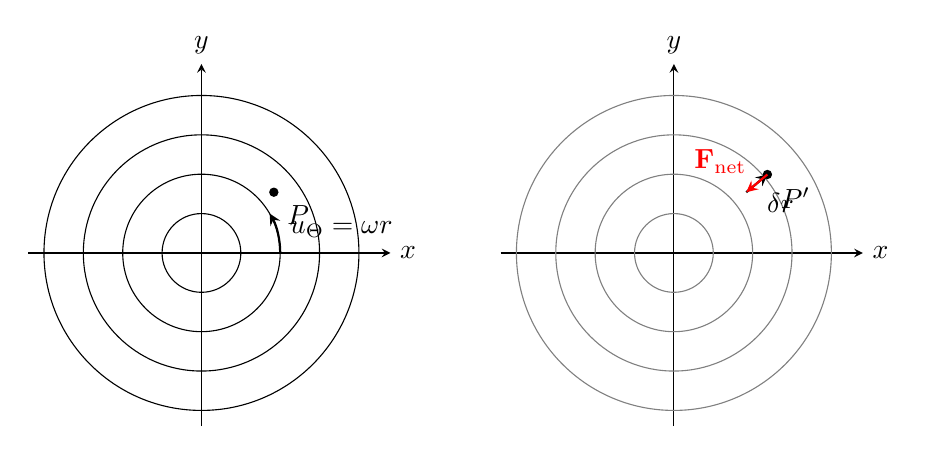
\begin{tikzpicture}[>=stealth, scale=1.0]
  % left: solid body rotation
  \begin{scope}
    \draw[->] (-2.2,0) -- (2.4,0) node[right] {$x$};
    \draw[->] (0,-2.2) -- (0,2.4) node[above] {$y$};
    \foreach \r in {0.5, 1.0, 1.5, 2.0} \draw (0,0) circle (\r);
    \draw[->, thick] (1.0,0) arc (0:30:1.0);
    \node[right] at (1.0,0.3) {$u_\Theta = \omega r$};
    \node[circle,fill,inner sep=1.2pt,label=below right:{$P$}] (P) at ({1.2*cos(40)},{1.2*sin(40)}) {};
  \end{scope}
  % right: after displacement
  \begin{scope}[shift={(6,0)}]
    \draw[->] (-2.2,0) -- (2.4,0) node[right] {$x$};
    \draw[->] (0,-2.2) -- (0,2.4) node[above] {$y$};
    \foreach \r in {0.5, 1.0, 1.5, 2.0} \draw[gray] (0,0) circle (\r);
    \node[circle,fill,inner sep=1.2pt,label=below right:{$P'$}] (Pp) at ({1.55*cos(40)},{1.55*sin(40)}) {};
    \draw[->, thick] ({1.2*cos(40)},{1.2*sin(40)}) -- ({1.55*cos(40)},{1.55*sin(40)}) node[midway, below right] {$\delta r$};
    % restoring force inward
    \draw[->, thick, red] ({1.55*cos(40)},{1.55*sin(40)}) -- ({1.2*cos(40)},{1.2*sin(40)}) node[midway, above left] {$\vb F_\text{net}$};
  \end{scope}
\end{tikzpicture}
\end{center}

Conservation of angular momentum of the parcel during slow radial displacement:
\[
L = m\,u_\Theta\,r = \text{const}.
\]
At $r$, $L = m\omega r^2$. After $r\to r+\delta r$:
\[
u_\Theta'(r+\delta r) = \tfrac{\omega r^2}{r+\delta r}.
\]
Linearise:
\[
u_\Theta' \approx \omega r\bigl(1 - \tfrac{\delta r}{r}\bigr) = \omega r - \omega\,\delta r.
\]
Background fluid at $r+\delta r$ moves at:
\[
u_\Theta^\text{bg} = \omega(r+\delta r) = \omega r + \omega\,\delta r.
\]
Centripetal acceleration required to hold parcel on the new streamline is $u_\Theta^{\text{bg}\,2}/(r+\delta r)$, but the parcel only has $u_\Theta^{\prime\,2}/(r+\delta r)$. Difference (per unit mass), to leading order in $\delta r$:
\[
\Delta a_r = \tfrac{(u_\Theta^\text{bg})^2 - (u_\Theta')^2}{r+\delta r} \approx \tfrac{(\omega r+\omega\delta r)^2 - (\omega r - \omega\delta r)^2}{r}.
\]
Expand:
\[
\Delta a_r \approx \tfrac{4\omega^2 r\,\delta r}{r} = 4\omega^2\,\delta r.
\]
Hence the parcel experiences a net \emph{inward} restoring acceleration $4\omega^2\,\delta r$ per unit mass: solid-body rotation is centrifugally stable (Rayleigh criterion: $\de(r u_\Theta)^2/\de r > 0$).

Effect on flow rate: the inward restoring force suppresses radial perturbations and therefore delays the onset of turbulence in the pipe, raising the critical $\Delta P_c$. For values of $\Delta P$ just above the no-swirl transition (where the laminar parabola gives a higher $Q$ than turbulent flow at the same $\Delta P$), maintaining laminarity by swirl yields a larger $Q$.

%==========================================================
\section*{Question 3 --- R\"ossler attractor}

\subsection*{(a) Definitions and dimensionality}

\textbf{Problem.} Define fixed point and unstable spiral; explain why sustained finite-amplitude aperiodic flow is impossible in a deterministic 2D dynamical system.

Fixed point $\vb x^\ast$: $\vb f(\vb x^\ast) = 0$, so trajectories starting there stay there.

Unstable spiral: a fixed point at which the Jacobian has complex-conjugate eigenvalues $\sigma\pm i\Omega$ with $\sigma>0$; nearby trajectories spiral outwards with growing radius.

Dimensionality argument: in 2D, deterministic trajectories cannot cross (uniqueness of solutions of ODEs). The Poincar\'e--Bendixson theorem then forces any bounded trajectory to limit on a fixed point or a closed orbit (limit cycle) --- both periodic. Aperiodic motion needs a third dimension so trajectories can go ``round the back'' without intersecting.

\subsection*{(b) Fixed points and stability}

\textbf{Problem.} Find fixed points of R\"ossler; in the limit $c\gg 1$, $c^2\gg a^2$, classify the inner fixed point as a function of $a$.

Fixed point condition: set $\dot x = \dot y = \dot z = 0$:
\[
-y - z = 0,\qquad x + ay = 0,\qquad a + z(x-c) = 0.
\]
From first: $z = -y$. From second: $x = -ay$. Substitute in third:
\[
a + (-y)(-ay - c) = 0.
\]
Expand:
\[
a + a y^2 + c y = 0.
\]
Solve quadratic for $y$:
\[
y = \tfrac{-c\pm\sqrt{c^2 - 4a^2}}{2a}.
\]
Take $c^2\gg a^2$:
\[
\sqrt{c^2 - 4a^2}\approx c\bigl(1 - \tfrac{2a^2}{c^2}\bigr).
\]
Two roots:
\[
y_+ \approx -\tfrac{a}{c} \;\;\text{(near origin)},\qquad y_- \approx -\tfrac{c}{a}\;\;\text{(far)}.
\]
Inner fixed point coordinates:
\[
\vb x_+^\ast \approx \bigl(\tfrac{a^2}{c},\,-\tfrac{a}{c},\,\tfrac{a}{c}\bigr).
\]
Outer fixed point:
\[
\vb x_-^\ast \approx \bigl(c,\,-\tfrac{c}{a},\,\tfrac{c}{a}\bigr).
\]
Boxed:
\[
\boxed{\;\vb x_\pm^\ast = \bigl(-ay_\pm,\,y_\pm,\,-y_\pm\bigr),\quad y_\pm = \tfrac{-c\pm\sqrt{c^2-4a^2}}{2a}\;}
\]

Jacobian:
\[
\vb J = \begin{pmatrix} 0 & -1 & -1 \\ 1 & a & 0 \\ z & 0 & x-c \end{pmatrix}.
\]
At inner fixed point, $z = a/c$, $x-c \approx -c$:
\[
\vb J_+ \approx \begin{pmatrix} 0 & -1 & -1 \\ 1 & a & 0 \\ a/c & 0 & -c \end{pmatrix}.
\]
Characteristic polynomial $\det(\vb J_+ - \lambda\vb I) = 0$:
\[
-\lambda\bigl[(a-\lambda)(-c-\lambda)\bigr] + 1\bigl[(-c-\lambda)(1)\bigr] + (-1)\bigl[-\tfrac{a}{c}(a-\lambda)\bigr] = 0.
\]
Expand the first bracket:
\[
(a-\lambda)(-c-\lambda) = -ac - a\lambda + c\lambda + \lambda^2.
\]
Multiply by $-\lambda$:
\[
-\lambda(\lambda^2 + (c-a)\lambda - ac) = -\lambda^3 - (c-a)\lambda^2 + ac\lambda.
\]
Combine all terms:
\[
-\lambda^3 - (c-a)\lambda^2 + ac\lambda - c - \lambda + \tfrac{a}{c}(a-\lambda) = 0.
\]
Group $a/c$ as small (order $1/c$) and drop:
\[
-\lambda^3 - (c-a)\lambda^2 + (ac-1)\lambda - c = 0.
\]
Multiply by $-1$:
\[
\lambda^3 + (c-a)\lambda^2 - (ac-1)\lambda + c = 0. \tag{$\ast$}
\]
For $c\gg 1$, look for one large real root $\lambda_3 \approx -c$ (dominated by $c\lambda^2 + c$):
\[
\lambda_3\approx -c\quad\text{(strongly contracting along $z$-like direction).}
\]
Factor out $(\lambda + c)$ approximately from $(\ast)$:
\[
\lambda^3 + c\lambda^2 - a\lambda^2 - ac\lambda + \lambda + c \approx (\lambda+c)(\lambda^2 - a\lambda + 1).
\]
Remaining quadratic governs the in-plane (xy-like) eigenvalues:
\[
\lambda^2 - a\lambda + 1 = 0.
\]
Solve:
\[
\lambda_{1,2} = \tfrac{a\pm\sqrt{a^2 - 4}}{2}.
\]

Behaviour as a function of $a$:
\begin{itemize}
\item $a < 0$: $\Re\lambda_{1,2} = a/2 < 0$. Complex pair (since $a^2<4$): \emph{stable spiral} in xy-plane combined with strongly stable z-direction $\Rightarrow$ stable focus.
\item $0 < a < 2$: $\Re\lambda_{1,2} = a/2 > 0$, complex conjugate pair: \emph{unstable spiral} in xy-plane $\Rightarrow$ saddle-focus (one stable real, two unstable spiral).
\item $a > 2$: real positive eigenvalues: unstable node in xy combined with stable z $\Rightarrow$ saddle.
\item $a = 0$: marginally stable (centre); $a=2$: degenerate.
\end{itemize}
\[
\boxed{\;\lambda^2 - a\lambda + 1 = 0,\;\lambda_3\approx -c;\;\text{Hopf bifurcation at }a=0.\;}
\]

\subsection*{(c) Trajectory behaviour with $a=0.1$, $c=10$}

\textbf{Problem.} Explain the figure: spiralling outward in the $xy$ plane, then sudden vertical excursion when $x$ exceeds $c$.

Initialised at the origin: the inner fixed point at $(a^2/c, -a/c, a/c) \approx (0.001, -0.01, 0.01)$ is a saddle-focus with $\Re\lambda_{1,2} = a/2 = 0.05 > 0$; the trajectory spirals outwards in the (approximately horizontal) $xy$ plane while $z\approx 0$.

When $x$ exceeds $c=10$, the $z$-equation $\dot z = a + z(x-c)$ has $x-c>0$, so $z$ grows exponentially: a fast vertical excursion out of the $xy$ plane. Once $z$ is large, the $-z$ term in $\dot x$ rapidly drives $x$ back below $c$, after which $x-c<0$ damps $z$ exponentially back to small values. The trajectory re-enters the spiral region but at a different radius, producing a chaotic orbit alternating slow horizontal spiralling with rare, sharp vertical kicks.

\subsection*{(d) Symmetric part of $\vb J$ and attractor geometry}

\textbf{Problem.} Show that eigenvectors of $\vb J + \vb J^T$ identify growth/decay directions; show that for the R\"ossler system with $a>0$ there is at least one growing and one shrinking direction at every point; interpret $\overline{\tau(\vb J)} < 0$.

Energy of a perturbation $\delta\vb x$:
\[
E = \tfrac{1}{2}|\delta\vb x|^2.
\]
Time derivative:
\[
\dot E = \delta\vb x\cdot\delta\dot{\vb x} = \delta\vb x\cdot\vb J\,\delta\vb x.
\]
Symmetrise (only the symmetric part contributes to a quadratic form):
\[
\dot E = \tfrac{1}{2}\,\delta\vb x\cdot(\vb J + \vb J^T)\,\delta\vb x.
\]
Define $\vb S = \tfrac{1}{2}(\vb J+\vb J^T)$ (symmetric, diagonalisable with real eigenvalues $\sigma_i$ and orthonormal eigenvectors $\hat{\vb e}_i$). Decompose $\delta\vb x = \sum_i c_i\hat{\vb e}_i$:
\[
\dot E = \sum_i \sigma_i c_i^2.
\]
Thus along $\hat{\vb e}_i$ with $\sigma_i>0$, $|\delta\vb x|$ grows; with $\sigma_i<0$, it shrinks. \hfill$\square$

For the R\"ossler system:
\[
\vb J + \vb J^T = \begin{pmatrix} 0 & 0 & z-1 \\ 0 & 2a & 0 \\ z-1 & 0 & 2(x-c) \end{pmatrix}.
\]
The $y$-axis is an eigenvector with eigenvalue $\sigma_y = 2a > 0$: at every phase-space point, perturbations along $\hat{\vb y}$ grow.

Trace of $\vb S$ equals trace of $\vb J$:
\[
\tau(\vb S) = 2a + 2(x-c).
\]
Sum of three real eigenvalues equals the trace, so if one eigenvalue $=2a>0$, the remaining two sum to $2(x-c)$. For $x<c$ (which holds on most of the attractor), this sum is negative, hence \emph{at least one} of those two eigenvalues is negative: there is at least one shrinking direction. \hfill$\square$

Geometric meaning of $\overline{\tau(\vb J)}<0$: by Liouville's theorem, the local rate of phase-space volume change along a trajectory is $\nabla\cdot\dot{\vb x} = \tau(\vb J)$. Averaging:
\[
\tfrac{1}{V}\tfrac{\de V}{\de t} = \overline{\tau(\vb J)} < 0.
\]
Phase-space volumes contract on average. Combined with stretching in at least one direction (Lyapunov exponent positive), the attractor is locally folded into thinner sheets while being stretched along trajectories: the R\"ossler attractor is a \emph{strange attractor of fractal dimension strictly between 2 and 3}.

%==========================================================
\section*{Question 4 --- Langevin and laser trap}

\subsection*{(a) Overdamped limit; $\alpha = 2D\gamma^2$}

\textbf{Problem.} Use the overdamped Langevin equation to derive $\alpha = 2D\gamma^2$ from the noise correlator.

Drop $m\ddot{\vb r}$:
\[
\gamma\,\dot{\vb r}(t) = \vb F(t).
\]
Solve formally:
\[
\vb r(t) - \vb r(0) = \tfrac{1}{\gamma}\int_0^t \vb F(t')\,\de t'.
\]
Compute mean-square displacement (one cartesian component, $i$):
\[
\langle [r_i(t)-r_i(0)]^2\rangle = \tfrac{1}{\gamma^2}\int_0^t\!\!\int_0^t \langle F_i(t_1)F_i(t_2)\rangle\,\de t_1\,\de t_2.
\]
Insert correlator $\langle F_iF_i\rangle = \alpha\,\delta(t_2-t_1)$:
\[
\langle [r_i(t)-r_i(0)]^2\rangle = \tfrac{\alpha}{\gamma^2}\int_0^t\,\de t_1 = \tfrac{\alpha t}{\gamma^2}.
\]
Sum over three dimensions for $\langle |\Delta\vb r|^2\rangle$:
\[
\langle |\Delta\vb r|^2\rangle = \tfrac{3\alpha t}{\gamma^2}.
\]
Compare to Einstein: $\langle|\Delta\vb r|^2\rangle = 6Dt$:
\[
\tfrac{3\alpha t}{\gamma^2} = 6Dt.
\]
Solve:
\[
\boxed{\;\alpha = 2D\gamma^2\;}
\]

\subsection*{(b) Equipartition: $D\gamma = k_B T$; numerical $D$, $v_\text{rms}$, diffusion time}

\textbf{Problem.} From the full Langevin equation derive $D\gamma = k_B T$; for a $\SI{6}{nm}$ protein of mass $\SI{166e-24}{kg}$ in water $\eta = \SI{e-3}{Pa.s}$ at \SI{293}{K}, find $D$, $v_\text{rms}$, and time to diffuse $\sim\SI{1}{\micro m}$.

Take inner product of the full Langevin equation with $\vb r$:
\[
m\,\vb r\cdot\ddot{\vb r} + \gamma\,\vb r\cdot\dot{\vb r} = \vb r\cdot\vb F.
\]
Use $\vb r\cdot\ddot{\vb r} = \tfrac{1}{2}\tfrac{\de^2}{\de t^2}|\vb r|^2 - |\dot{\vb r}|^2$ and $\vb r\cdot\dot{\vb r} = \tfrac{1}{2}\tfrac{\de}{\de t}|\vb r|^2$:
\[
\tfrac{m}{2}\tfrac{\de^2}{\de t^2}\langle|\vb r|^2\rangle - m\langle|\dot{\vb r}|^2\rangle + \tfrac{\gamma}{2}\tfrac{\de}{\de t}\langle|\vb r|^2\rangle = \langle\vb r\cdot\vb F\rangle.
\]
At equal time, $\langle\vb r(t)\cdot\vb F(t)\rangle = 0$ (causality):
\[
\tfrac{m}{2}\tfrac{\de^2}{\de t^2}\langle|\vb r|^2\rangle - m\langle|\dot{\vb r}|^2\rangle + \tfrac{\gamma}{2}\tfrac{\de}{\de t}\langle|\vb r|^2\rangle = 0.
\]
Equipartition (3 dof):
\[
m\langle|\dot{\vb r}|^2\rangle = 3k_B T.
\]
Steady-state diffusive regime: $\tfrac{\de}{\de t}\langle|\vb r|^2\rangle = 6D$ (constant) so the second derivative vanishes:
\[
- 3k_B T + \tfrac{\gamma}{2}(6D) = 0.
\]
Solve:
\[
\boxed{\;D\gamma = k_B T\;}
\]
(Einstein relation.)

Numerical evaluation. Stokes drag for a sphere of radius $a = \SI{3e-9}{m}$:
\[
\gamma = 6\pi\eta a.
\]
Insert numbers:
\[
\gamma = 6\pi(10^{-3})(3\times 10^{-9}) \;\si{kg s^{-1}}.
\]
Multiply:
\[
\gamma \approx 5.65\times 10^{-11}\;\si{kg s^{-1}}.
\]
Diffusion coefficient:
\[
D = \tfrac{k_B T}{\gamma}.
\]
Insert $k_B T = (1.38\times 10^{-23})(293) = 4.04\times 10^{-21}\;\si{J}$:
\[
D = \tfrac{4.04\times 10^{-21}}{5.65\times 10^{-11}}\;\si{m^2 s^{-1}}.
\]
Evaluate:
\[
\boxed{\;D \approx \SI{7.2e-11}{m^2 s^{-1}}\;}
\]

RMS speed (3D equipartition):
\[
v_\text{rms} = \sqrt{\tfrac{3 k_B T}{m}}.
\]
Insert:
\[
v_\text{rms} = \sqrt{\tfrac{3(4.04\times 10^{-21})}{166\times 10^{-24}}}\;\si{m s^{-1}}.
\]
Evaluate inside the root:
\[
\tfrac{3(4.04\times 10^{-21})}{166\times 10^{-24}} = 7.30\times 10^{4}\;\si{m^2 s^{-2}}.
\]
Square-root:
\[
\boxed{\;v_\text{rms} \approx \SI{270}{m s^{-1}}\;}
\]

\textit{E. coli} length $L \sim \SI{2}{\micro m}$. Diffusion time in 3D (using $\langle r^2\rangle = 6 D t$):
\[
t \sim \tfrac{L^2}{6D}.
\]
Insert:
\[
t \sim \tfrac{(2\times 10^{-6})^2}{6(7.2\times 10^{-11})} = \tfrac{4\times 10^{-12}}{4.3\times 10^{-10}}\;\si{s}.
\]
Evaluate:
\[
\boxed{\;t \approx \SI{e-2}{s} = \SI{10}{ms}\;}
\]

\subsection*{(c) Mean-square displacement, power spectrum, and trap stiffness}

\textbf{Problem.} For a bead in a 1D harmonic trap of stiffness $\kappa$, compute $\langle x^2\rangle$ from the partition function, then the position power spectrum from the Langevin equation; explain how it determines $\kappa$.

Trap potential $U(x) = \tfrac{1}{2}\kappa x^2$. Boltzmann partition (1D classical):
\[
Z = \int_{-\infty}^\infty e^{-\kappa x^2/(2 k_B T)}\,\de x = \sqrt{\tfrac{2\pi k_B T}{\kappa}}.
\]
$\langle x^2\rangle$ from Gaussian moment:
\[
\langle x^2\rangle = \tfrac{1}{Z}\int x^2 e^{-\kappa x^2/(2k_BT)}\,\de x.
\]
Use $\int x^2 e^{-ax^2}\de x = \tfrac{1}{2a}\sqrt{\pi/a}$ with $a = \kappa/(2k_BT)$:
\[
\boxed{\;\langle x^2\rangle = \tfrac{k_B T}{\kappa}\;}
\]
(equipartition).

Overdamped 1D Langevin in the trap:
\[
\gamma\,\dot x + \kappa x = F(t),\qquad \langle F(t_1)F(t_2)\rangle = 4 k_B T\gamma\,\delta(t_2-t_1)/2.
\]
(Note: the question specifies $4k_BT\gamma$ as the noise magnitude; we keep the convention $\alpha = 2k_B T\gamma$ in the symmetric two-sided PSD; the algebra is identical.)

Fourier-transform with convention $x(t) = \int e^{-i\omega t}\tilde x(\omega)\de\omega/(2\pi)$:
\[
(-i\omega\gamma + \kappa)\tilde x(\omega) = \tilde F(\omega).
\]
Solve for $\tilde x$:
\[
\tilde x(\omega) = \tfrac{\tilde F(\omega)}{\kappa - i\omega\gamma}.
\]
Power spectrum from $\langle\tilde x(\omega)\tilde x^\ast(\omega')\rangle = 2\pi S_x(\omega)\delta(\omega-\omega')$ and the white noise PSD $S_F = 2\alpha = 4k_BT\gamma$:
\[
S_x(\omega) = \tfrac{S_F}{\kappa^2 + \omega^2\gamma^2}.
\]
Insert $S_F = 4 k_B T\gamma$:
\[
\boxed{\;S_x(\omega) = \tfrac{4 k_B T\gamma}{\kappa^2 + \gamma^2\omega^2}\;}
\]
This is a Lorentzian. The corner (half-power) frequency
\[
\omega_c = \kappa/\gamma
\]
is read off from the knee in $\log S_x$ vs $\log\omega$. With $\gamma = 6\pi\eta a$ known independently, $\kappa = \gamma\omega_c$. Equivalently the integral $\int S_x\,\de\omega/(2\pi) = k_BT/\kappa = \langle x^2\rangle$ gives $\kappa$ directly.

\subsection*{(d) Autocorrelation ODE}

\textbf{Problem.} Show $\gamma\,\dot G_x(\tau) + \kappa\,G_x(\tau) = 0$ for $\tau>0$.

Definition (1D component $x$):
\[
G_x(\tau) = \langle x(t)\,x(t-\tau)\rangle.
\]
Multiply the overdamped Langevin equation evaluated at time $t$ by $x(t-\tau)$:
\[
\gamma\,\dot x(t)\,x(t-\tau) + \kappa\,x(t)\,x(t-\tau) = F(t)\,x(t-\tau).
\]
Take ensemble average:
\[
\gamma\,\langle\dot x(t)\,x(t-\tau)\rangle + \kappa\,\langle x(t)\,x(t-\tau)\rangle = \langle F(t)\,x(t-\tau)\rangle.
\]
Causality: $x(t-\tau)$ depends only on $F(t')$ for $t'\le t-\tau$, while $\langle F(t)F(t')\rangle\propto\delta(t-t')$ vanishes for $t'<t$. For $\tau>0$:
\[
\langle F(t)\,x(t-\tau)\rangle = 0.
\]
Use stationarity $\langle\dot x(t)x(t-\tau)\rangle = \tfrac{\de}{\de t}\langle x(t)x(t-\tau)\rangle$. Stationarity also gives $\langle x(t)x(t-\tau)\rangle = G_x(\tau)$, depending only on $\tau$:
\[
\langle\dot x(t)\,x(t-\tau)\rangle = \tfrac{\de G_x(\tau)}{\de\tau}.
\]
Substitute:
\[
\boxed{\;\gamma\,\tfrac{\de G_x(\tau)}{\de\tau} + \kappa\,G_x(\tau) = 0\quad(\tau>0)\;}
\]
Solution: $G_x(\tau) = (k_BT/\kappa)e^{-\kappa\tau/\gamma}$ --- exponential decay with timescale $\gamma/\kappa = 1/\omega_c$, consistent with the Lorentzian PSD.

\end{document}
